\section{Khảo sát thực trạng tra cứu thủ tục
hành
chính}

Nguồn khảo sát chính của đồ án là Cổng Dịch vụ công tỉnh Lai Châu và các
trang chi tiết thủ tục có cấu trúc dữ liệu công khai. Tại thời điểm hoàn
thiện đồ án, dữ liệu trong báo cáo được sử dụng như bộ dữ liệu tra cứu
phục vụ thử nghiệm, không thay thế thông tin pháp lý đang có hiệu lực
trên hệ thống chính thức.

\begin{figure}[H]
\centering
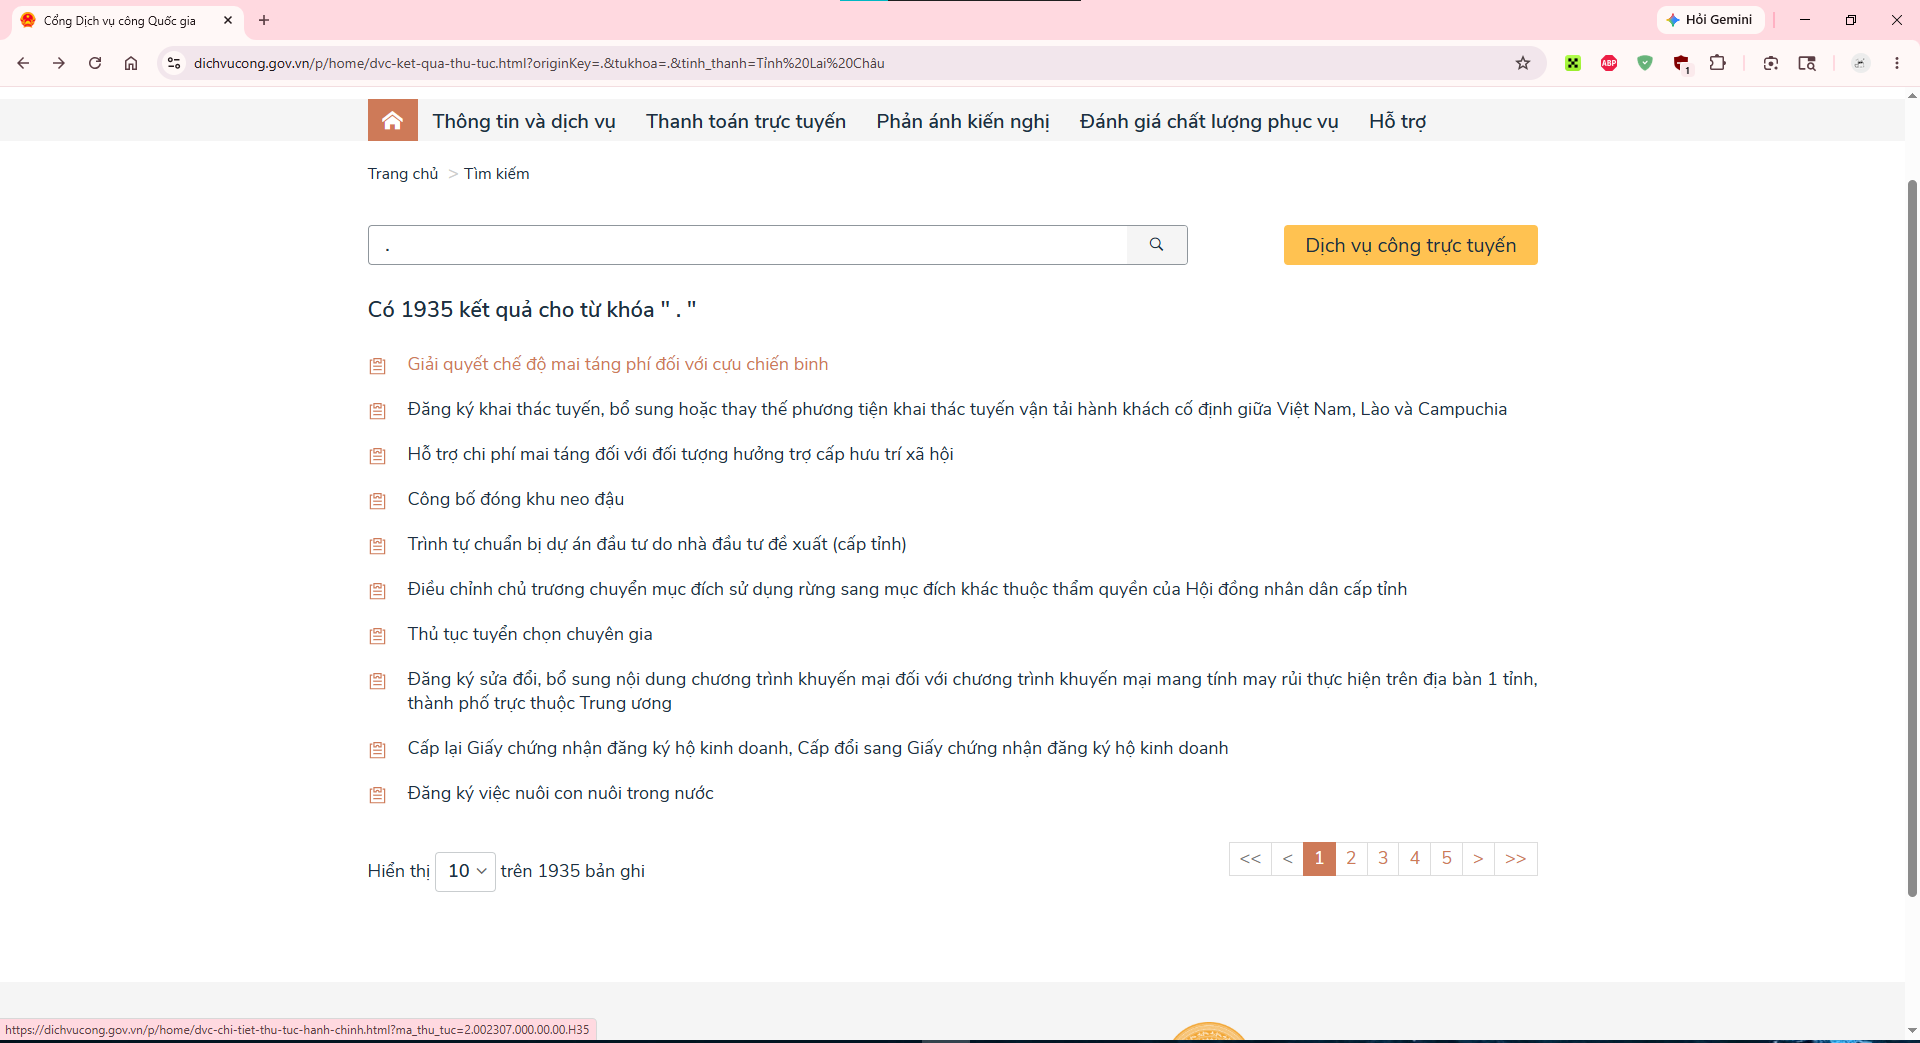
\includegraphics[width=0.92\textwidth]{tai_nguyen/media/image1.png}
\caption{Ảnh màn hình trang tra cứu TTHC trên Cổng Dịch vụ công tỉnh Lai Châu}
\label{fig:2-1}
\end{figure}

\begin{figure}[H]
\centering
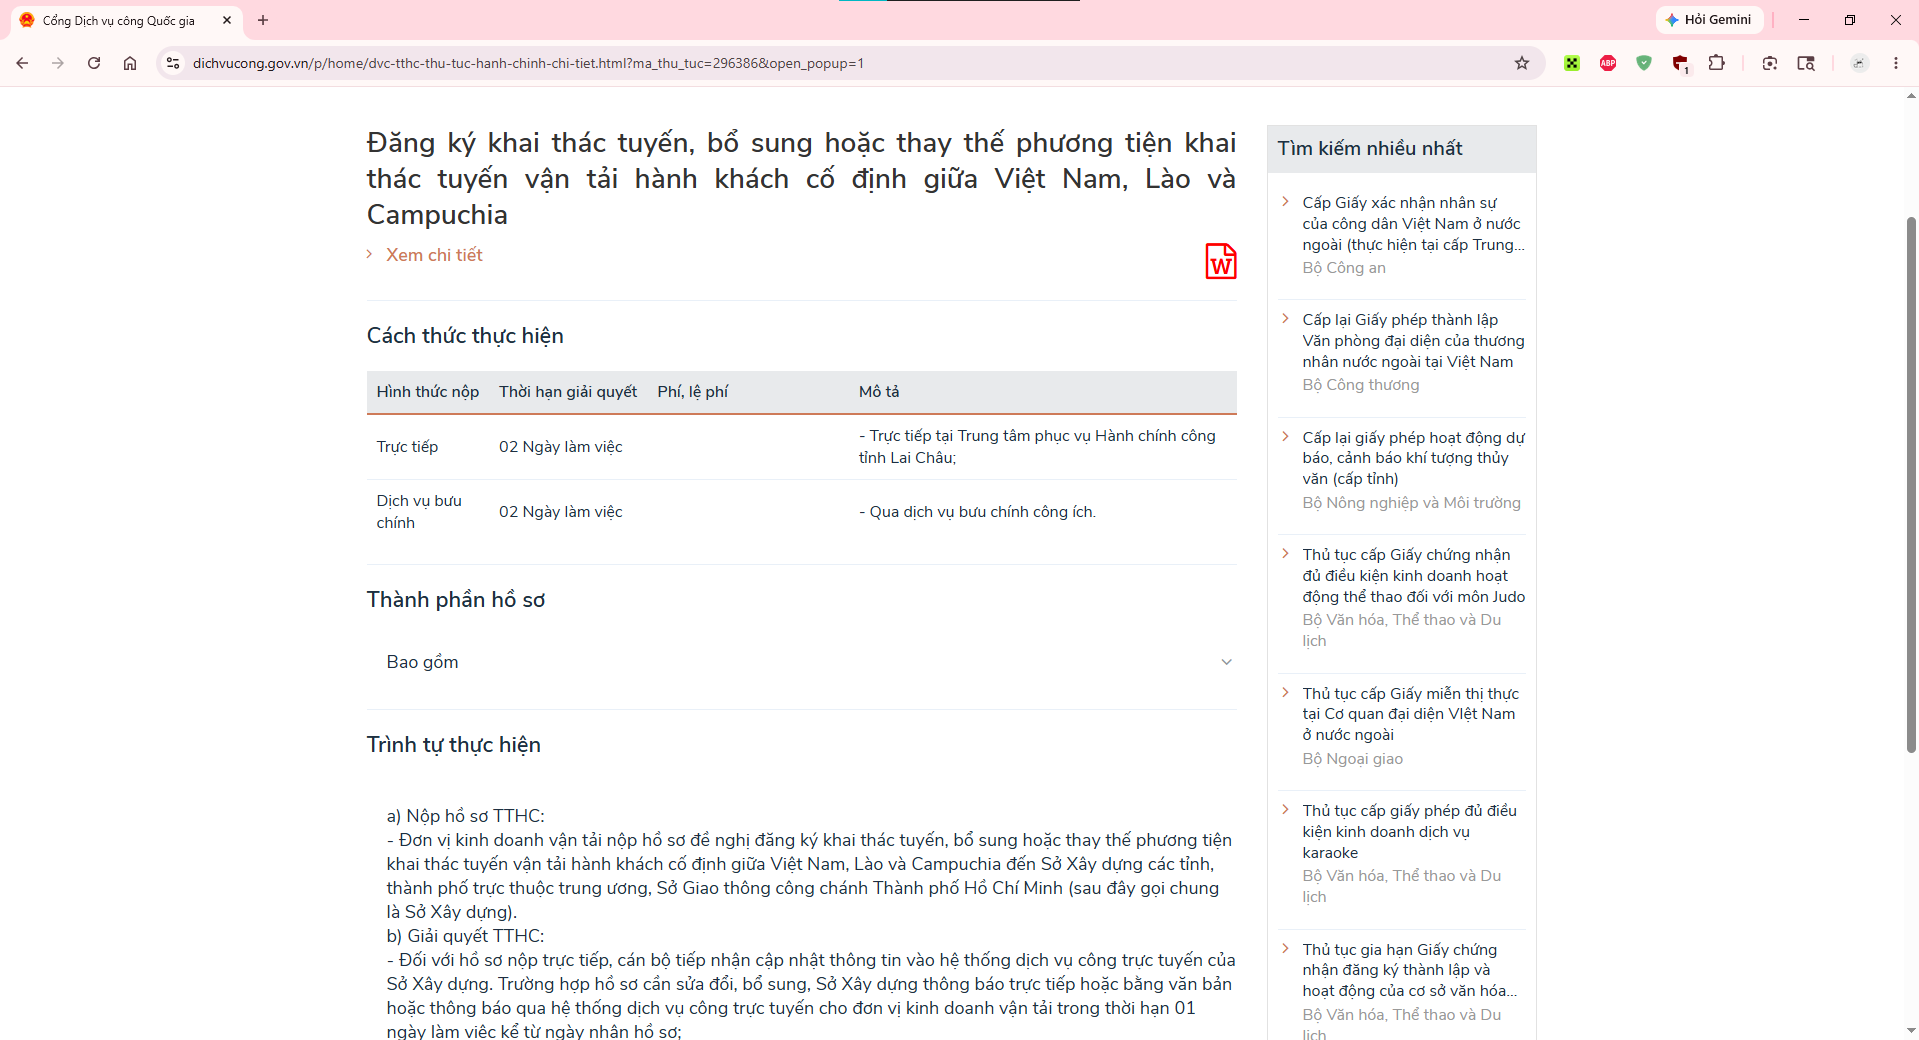
\includegraphics[width=0.92\textwidth]{tai_nguyen/media/image2.png}
\caption{Ảnh màn hình trang chi tiết một TTHC trước khi chuẩn hóa dữ liệu}
\label{fig:2-2}
\end{figure}

\begin{longtable}[]{|
  >{\raggedright\arraybackslash}p{(\columnwidth - 2\tabcolsep) * \real{0.2491}}|
  >{\raggedright\arraybackslash}p{(\columnwidth - 2\tabcolsep) * \real{0.7509}}|}
\caption{Minh chứng nguồn dữ liệu và xử lý dữ liệu đầu vào}\\
\hline
\begin{minipage}[b]{\linewidth}\raggedright
\textbf{Nội dung}
\end{minipage} & \begin{minipage}[b]{\linewidth}\raggedright
\textbf{Mô tả trong đồ án}
\end{minipage} \\
\hline
\endfirsthead
\continuedcaption{Minh chứng nguồn dữ liệu và xử lý dữ liệu đầu vào}
\hline
\begin{minipage}[b]{\linewidth}\raggedright
\textbf{Nội dung}
\end{minipage} & \begin{minipage}[b]{\linewidth}\raggedright
\textbf{Mô tả trong đồ án}
\end{minipage} \\
\hline
\endhead
\hline
\endlastfoot
Nguồn dữ liệu & Cổng Dịch vụ công tỉnh Lai Châu và trang chi tiết thủ
tục hành chính công khai. \\
\hline
Thời điểm chốt dữ liệu & Tháng 10/05/2026, phục vụ phiên bản thử nghiệm
của đồ án. \\
\hline
Định dạng ban đầu & Dữ liệu chi tiết thủ tục dạng văn bản/bảng trên
trang web, sau đó chuẩn hóa sang JSON. \\
\hline
Quy mô dữ liệu & 1950 thủ tục, 176 lĩnh vực, 1950 nhóm thực thể nhận
diện tên thủ tục. \\
\hline
Kiểm tra trùng/lỗi & Không ghi nhận mã thủ tục trùng; loại bỏ giá trị
rỗng/không quy định; chuẩn hóa cách biểu diễn phí, lệ phí và thành phần
hồ sơ. \\
\hline
\end{longtable}

Từ khảo sát thực tế, các khó khăn chính của người dùng nằm ở việc không
biết đúng tên thủ tục, nội dung thủ tục dài, văn phong pháp lý khó đọc
và thông tin cần tìm nằm rải rác. Điều này dẫn tới yêu cầu hệ thống phải
hỗ trợ hỏi bằng ngôn ngữ tự nhiên, truy xuất theo ngữ nghĩa và trình bày
lại câu trả lời ngắn gọn hơn văn bản gốc.

\begin{longtable}[]{|
  >{\raggedright\arraybackslash}p{(\columnwidth - 4\tabcolsep) * \real{0.2497}}|
  >{\raggedright\arraybackslash}p{(\columnwidth - 4\tabcolsep) * \real{0.3409}}|
  >{\raggedright\arraybackslash}p{(\columnwidth - 4\tabcolsep) * \real{0.4094}}|}
\caption{Tổng hợp vấn đề trong quá trình tra cứu TTHC}\\
\hline
\begin{minipage}[b]{\linewidth}\raggedright
\textbf{Nhóm vấn đề}
\end{minipage} & \begin{minipage}[b]{\linewidth}\raggedright
\textbf{Biểu hiện}
\end{minipage} & \begin{minipage}[b]{\linewidth}\raggedright
\textbf{Tác động đến thiết kế hệ thống}
\end{minipage} \\
\hline
\endfirsthead
\continuedcaption{Tổng hợp vấn đề trong quá trình tra cứu TTHC}
\hline
\begin{minipage}[b]{\linewidth}\raggedright
\textbf{Nhóm vấn đề}
\end{minipage} & \begin{minipage}[b]{\linewidth}\raggedright
\textbf{Biểu hiện}
\end{minipage} & \begin{minipage}[b]{\linewidth}\raggedright
\textbf{Tác động đến thiết kế hệ thống}
\end{minipage} \\
\hline
\endhead
\hline
\endlastfoot
Tên thủ tục khó nhớ & Người dân mô tả nhu cầu bằng ngôn ngữ đời thường.
& Cần nhận diện biến thể từ khóa và tìm kiếm theo ngữ nghĩa. \\
\hline
Thông tin nằm rải rác & Hồ sơ, phí, thời hạn, cơ quan tiếp nhận ở các
mục khác nhau. & Cần chunk dữ liệu theo nhóm thông tin. \\
\hline
Văn phong pháp lý & Nhiều đoạn dài, khó đọc với người dùng phổ thông. &
Cần LLM diễn giải lại nhưng phải bám nguồn. \\
\hline
Dữ liệu thay đổi & Thủ tục có thể được cập nhật theo văn bản mới. & Cần
cơ chế cập nhật JSON và build lại VectorDB. \\
\hline
Độ chính xác cao & Trả lời sai có thể làm người dân chuẩn bị sai hồ sơ.
& Prompt phải ràng buộc, không trả lời ngoài context. \\
\hline
\end{longtable}

\section{Phân tích dữ liệu đầu
vào}

Dữ liệu đầu vào chính của hệ thống là file procedures.json, được chuẩn
hóa từ các trang chi tiết TTHC. Mỗi thủ tục gồm mã thủ tục, tên thủ tục
và phần content chứa các trường nghiệp vụ như lĩnh vực, đối tượng thực
hiện, cơ quan thực hiện, cách thức thực hiện, thành phần hồ sơ, thời hạn
giải quyết, phí, lệ phí, kết quả thực hiện và căn cứ pháp lý.

Bộ dữ liệu thử nghiệm được chốt trong tháng 05/2026, gồm 1950 TTHC thuộc
176 lĩnh vực. Trong quá trình làm sạch, các bản ghi được kiểm tra theo
mã thủ tục và tên thủ tục để hạn chế trùng lặp. Các giá trị rỗng, không
quy định hoặc không có thông tin được xử lý riêng để tránh đưa nội dung
nhiễu vào ChromaDB.

\begin{longtable}[]{|
  >{\raggedright\arraybackslash}p{(\columnwidth - 2\tabcolsep) * \real{0.2967}}|
  >{\raggedright\arraybackslash}p{(\columnwidth - 2\tabcolsep) * \real{0.7033}}|}
\caption{Ví dụ thủ tục thật trước và sau khi đưa vào hệ thống}\\
\hline
\begin{minipage}[b]{\linewidth}\raggedright
\textbf{Trạng thái dữ liệu}
\end{minipage} & \begin{minipage}[b]{\linewidth}\raggedright
\textbf{Ví dụ mô tả}
\end{minipage} \\
\hline
\endfirsthead
\continuedcaption{Ví dụ thủ tục thật trước và sau khi đưa vào hệ thống}
\hline
\begin{minipage}[b]{\linewidth}\raggedright
\textbf{Trạng thái dữ liệu}
\end{minipage} & \begin{minipage}[b]{\linewidth}\raggedright
\textbf{Ví dụ mô tả}
\end{minipage} \\
\hline
\endhead
\hline
\endlastfoot
Trên cổng dịch vụ công & Người dùng phải đọc trang chi tiết thủ tục, tự
tìm các mục hồ sơ, thời hạn, cơ quan thực hiện và căn cứ pháp lý. \\
\hline
Trong procedures.json & Thông tin được lưu theo các trường có cấu trúc:
id, name, content, trong đó content chứa Lĩnh vực, Cách thức thực hiện,
Thành phần hồ sơ, Phí, Lệ phí, Căn cứ pháp lý... \\
\hline
Trong ChromaDB & Mỗi nhóm thông tin được chuyển thành chunk riêng, ví dụ
chunk tổng quan, chunk cách thức thực hiện, chunk thành phần hồ sơ và
chunk căn cứ pháp lý. \\
\hline
Khi hỏi chatbot & Câu hỏi ``mai táng phí cựu chiến binh cần hồ sơ gì?''
được ánh xạ tới chunk Thành phần hồ sơ thay vì trả lại toàn bộ thủ
tục. \\
\hline
\end{longtable}

\begin{longtable}[]{|
  >{\raggedright\arraybackslash}p{(\columnwidth - 4\tabcolsep) * \real{0.2181}}|
  >{\raggedright\arraybackslash}p{(\columnwidth - 4\tabcolsep) * \real{0.2336}}|
  >{\raggedright\arraybackslash}p{(\columnwidth - 4\tabcolsep) * \real{0.5483}}|}
\caption{Thống kê dữ liệu đầu vào phục vụ hệ thống RAG}\\
\hline
\begin{minipage}[b]{\linewidth}\raggedright
\textbf{Loại dữ liệu}
\end{minipage} & \begin{minipage}[b]{\linewidth}\raggedright
\textbf{Số lượng/quy mô}
\end{minipage} & \begin{minipage}[b]{\linewidth}\raggedright
\textbf{Vai trò trong hệ thống}
\end{minipage} \\
\hline
\endfirsthead
\continuedcaption{Thống kê dữ liệu đầu vào phục vụ hệ thống RAG}
\hline
\begin{minipage}[b]{\linewidth}\raggedright
\textbf{Loại dữ liệu}
\end{minipage} & \begin{minipage}[b]{\linewidth}\raggedright
\textbf{Số lượng/quy mô}
\end{minipage} & \begin{minipage}[b]{\linewidth}\raggedright
\textbf{Vai trò trong hệ thống}
\end{minipage} \\
\hline
\endhead
\hline
\endlastfoot
Thủ tục hành chính & 1950 thủ tục & Dữ liệu gốc để tra cứu và sinh câu
trả lời. \\
\hline
Lĩnh vực thủ tục & 176 lĩnh vực & Hỗ trợ lọc, nhóm và phân tích dữ liệu
theo nghiệp vụ. \\
\hline
Thực thể tên thủ tục & 1950 nhóm thực thể & Nhận diện tên thủ tục và
biến thể từ khóa trong câu hỏi. \\
\hline
Intent hội thoại & 19 intent & Xử lý chào hỏi, cảm ơn, câu hỏi chung và
ngoài phạm vi. \\
\hline
Nhóm từ đồng nghĩa & 10 nhóm & Chuẩn hóa cách người dùng hỏi về hồ sơ,
phí, thời hạn, cơ quan, pháp lý. \\
\hline
Semantic chunk & Khoảng 30125 chunk & Lưu trong ChromaDB để truy xuất
theo ngữ nghĩa. \\
\hline
\end{longtable}

\emph{Các số liệu trong bảng được tổng hợp từ bộ dữ liệu đã chuẩn hóa
của hệ thống. Chi tiết thống kê dữ liệu thử nghiệm được trình bày tại
Phụ lục C.}

Khi build kho tri thức thử nghiệm, semantic chunker tạo các chunk từ dữ
liệu nguồn. Các chunk được phân nhóm thành tổng quan, cách thức thực
hiện, thành phần hồ sơ, căn cứ pháp lý và các trường đơn giản. Mỗi chunk
gắn metadata để pipeline có thể lọc theo thủ tục, lĩnh vực hoặc field
trước khi đưa vào LLM.

\section{Phân tích bài toán và phạm vi hệ
thống}

Bài toán của đề tài là tạo ra một lớp hỗ trợ tra cứu các TTHC bằng hội
thoại. Hệ thống không thay thế cổng dịch vụ công, không tiếp nhận hồ sơ
chính thức, không xử lý thanh toán và không thay thế thẩm quyền chuyên
môn của cán bộ hành chính. Phạm vi phù hợp của hệ thống là hỗ trợ người
dân tìm đúng thông tin cần biết trước khi chuẩn bị hồ sơ.

Người dùng chính gồm người dân và quản trị viên. Người dân sử dụng
chatbot để hỏi thông tin, tra cứu thủ tục, xem chi tiết thủ tục và xem
lại lịch sử hội thoại. Quản trị viên dùng dashboard để quản lý dữ liệu
thủ tục, theo dõi lịch sử, đồng bộ lại vector database và quản lý quyền
admin. Các dịch vụ như Firebase, Firestore, ChromaDB và LLM là thành
phần hỗ trợ kỹ thuật trong luồng xử lý.

\begin{longtable}[]{|
  >{\raggedright\arraybackslash}p{(\columnwidth - 4\tabcolsep) * \real{0.1249}}|
  >{\raggedright\arraybackslash}p{(\columnwidth - 4\tabcolsep) * \real{0.4381}}|
  >{\raggedright\arraybackslash}p{(\columnwidth - 4\tabcolsep) * \real{0.4370}}|}
\caption{Phạm vi thực hiện của hệ thống}\\
\hline
\begin{minipage}[b]{\linewidth}\raggedright
\textbf{Nội dung}
\end{minipage} & \begin{minipage}[b]{\linewidth}\raggedright
\textbf{Trong phạm vi đồ án}
\end{minipage} & \begin{minipage}[b]{\linewidth}\raggedright
\textbf{Ngoài phạm vi đồ án}
\end{minipage} \\
\hline
\endfirsthead
\continuedcaption{Phạm vi thực hiện của hệ thống}
\hline
\begin{minipage}[b]{\linewidth}\raggedright
\textbf{Nội dung}
\end{minipage} & \begin{minipage}[b]{\linewidth}\raggedright
\textbf{Trong phạm vi đồ án}
\end{minipage} & \begin{minipage}[b]{\linewidth}\raggedright
\textbf{Ngoài phạm vi đồ án}
\end{minipage} \\
\hline
\endhead
\hline
\endlastfoot
Tra cứu thông tin & Hỏi đáp về hồ sơ, thời hạn, phí/lệ phí, cơ quan, kết
quả, căn cứ pháp lý. & Không xác nhận tính hợp lệ cuối cùng của hồ sơ
như cán bộ chuyên môn. \\
\hline
Xem chi tiết thủ tục & Hiển thị/tra cứu thông tin chi tiết của một thủ
tục trong kho dữ liệu đã nạp. & Không thay thế văn bản gốc hoặc quyết
định công bố chính thức. \\
\hline
Tương tác & Hỏi đáp văn bản tiếng Việt qua giao diện web. & Chưa xử lý
giọng nói, ảnh giấy tờ hoặc OCR. \\
\hline
Dữ liệu & Sử dụng procedures.json và các file hỗ trợ entities, synonyms,
intents, codes. & Chưa kết nối trực tiếp toàn bộ hệ thống nghiệp vụ của
cơ quan nhà nước. \\
\hline
Triển khai & Chạy local, hosting frontend, backend thử nghiệm qua
server/ngrok. & Chưa vận hành như dịch vụ công chính thức ở quy mô
tỉnh. \\
\hline
\end{longtable}

\section{Phân tích tác nhân và nhu cầu sử
dụng}

Hai tác nhân trực tiếp là người dùng và quản trị viên. Người dùng quan
tâm đến tra cứu, xem chi tiết thủ tục, hỏi đáp chatbot và xem lại lịch
sử. Quản trị viên quan tâm đến quản lý dữ liệu, đồng bộ VectorDB, giám
sát hệ thống và quản lý quyền. Các thành phần Firebase Authentication,
Firestore, ChromaDB và LLM được xem là hệ thống phụ trợ tham gia vào quá
trình thực hiện nghiệp vụ.

\begin{longtable}[]{|
  >{\raggedright\arraybackslash}p{(\columnwidth - 4\tabcolsep) * \real{0.1797}}|
  >{\raggedright\arraybackslash}p{(\columnwidth - 4\tabcolsep) * \real{0.4507}}|
  >{\raggedright\arraybackslash}p{(\columnwidth - 4\tabcolsep) * \real{0.3695}}|}
\caption{Tác nhân và nhu cầu sử dụng}\\
\hline
\begin{minipage}[b]{\linewidth}\raggedright
\textbf{Tác nhân}
\end{minipage} & \begin{minipage}[b]{\linewidth}\raggedright
\textbf{Use Case chính}
\end{minipage} & \begin{minipage}[b]{\linewidth}\raggedright
\textbf{Vai trò}
\end{minipage} \\
\hline
\endfirsthead
\continuedcaption{Tác nhân và nhu cầu sử dụng}
\hline
\begin{minipage}[b]{\linewidth}\raggedright
\textbf{Tác nhân}
\end{minipage} & \begin{minipage}[b]{\linewidth}\raggedright
\textbf{Use Case chính}
\end{minipage} & \begin{minipage}[b]{\linewidth}\raggedright
\textbf{Vai trò}
\end{minipage} \\
\hline
\endhead
\hline
\endlastfoot
Người dùng & UC01 Đăng nhập; UC02 Tra cứu thủ tục; UC03 Xem chi tiết thủ
tục; UC04 Hỏi đáp chatbot; UC05 Xem lịch sử & Tìm hiểu thông tin thủ tục
và quản lý lịch sử hỏi đáp cá nhân. \\
\hline
Quản trị viên & UC06 Quản lý dữ liệu; UC07 Đồng bộ VectorDB; UC08 Quản
lý admin; UC09 Chuyển văn bản sang JSON; UC10 Giám sát hệ thống & Vận
hành kho dữ liệu và theo dõi hoạt động chatbot. \\
\hline
Firebase Auth & Xác thực token & Cung cấp định danh để backend kiểm tra
quyền truy cập. \\
\hline
Firestore & Lưu sessions, messages, OTP, settings & Lưu dữ liệu nghiệp
vụ và cấu hình. \\
\hline
ChromaDB & Truy xuất vector & Lưu embedding và metadata của các chunk
thủ tục. \\
\hline
LLM & Sinh câu trả lời, hỗ trợ JSON & Diễn giải context RAG và hỗ trợ
admin tạo dữ liệu ban đầu. \\
\hline
\end{longtable}

\section{Phân tích quy trình nghiệp
vụ}

Các quy trình nghiệp vụ được phân tách theo ba nhóm chính: quy trình
người dân tra cứu thủ tục, quy trình hỏi đáp bằng chatbot và quy trình
quản trị dữ liệu TTHC. Cách tách này giúp thể hiện rõ hệ thống không chỉ
là một chatbot trả lời câu hỏi mà còn gồm lớp tra cứu có cấu trúc và lớp
vận hành kho tri thức.

\subsection{Quy trình người dân tra cứu thủ tục hành
chính}
Quy trình tra cứu truyền thống trong phạm vi hệ thống bắt đầu khi người
dân nhập từ khóa hoặc nhu cầu thực tế. Frontend gửi yêu cầu tìm kiếm,
backend chuẩn hóa từ khóa và đối chiếu với dữ liệu thủ tục theo tên,
lĩnh vực hoặc metadata. Kết quả trả về là danh sách thủ tục liên quan để
người dùng mở chi tiết hoặc tiếp tục hỏi chatbot.

\begin{itemize}
\item
  Bước 1: Người dân nhập từ khóa, tên thủ tục hoặc mô tả nhu cầu.
\item
  Bước 2: Hệ thống chuẩn hóa truy vấn và tìm thủ tục liên quan trong kho
  dữ liệu.
\item
  Bước 3: Frontend hiển thị danh sách thủ tục phù hợp.
\item
  Bước 4: Người dân chọn một thủ tục để xem thông tin chi tiết hoặc
  chuyển sang hỏi chatbot.
\end{itemize}

\subsection{Quy trình hỏi đáp thủ tục hành chính bằng
chatbot}
Quy trình hỏi đáp được mô tả theo hướng BPMN. Sơ đồ cần có pool/lane,
start event, end event, task, gateway và data store để thể hiện rõ vai
trò của người dân, frontend, backend, kho tri thức và mô hình AI. Trong
bản Word này, sơ đồ BPMN hiện có được chuyển sang đúng mục 2.5.2 để khớp
với luồng hỏi đáp bằng chatbot.

\begin{figure}[H]
\centering
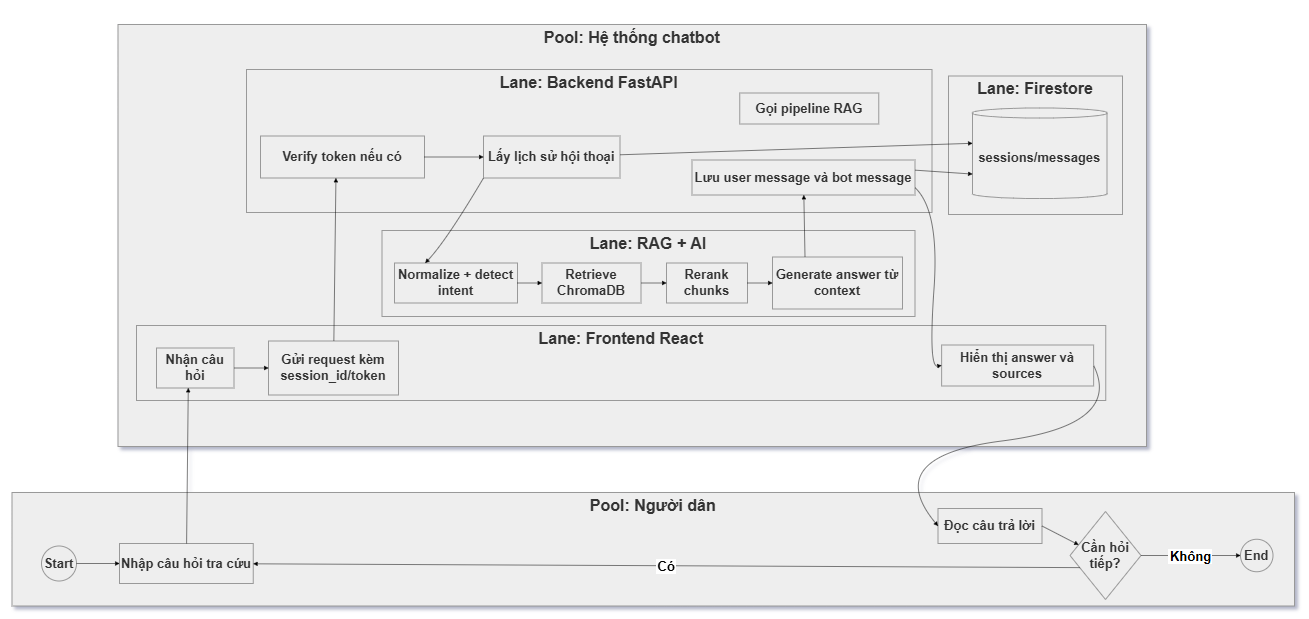
\includegraphics[width=0.92\textwidth]{tai_nguyen/media/image3.png}
\caption{Sơ đồ BPMN quy trình hỏi đáp TTHC bằng chatbot}
\label{fig:2-3}
\end{figure}

Quy trình bắt đầu từ nhu cầu tra cứu của người dân. Sau khi người dân
nhập câu hỏi, frontend gửi request đến backend. Backend kiểm tra xác
thực, lấy lịch sử hội thoại nếu có, gọi pipeline RAG để truy xuất dữ
liệu từ ChromaDB, xếp hạng lại kết quả và đưa context cho LLM sinh câu
trả lời. Sau khi trả kết quả, hệ thống lưu câu hỏi và câu trả lời vào
Firestore.

\subsection{Quy trình quản trị dữ liệu thủ tục hành
chính}
Quy trình quản trị dữ liệu được thực hiện bởi tài khoản có quyền admin.
Quản trị viên có thể thêm, sửa, xóa dữ liệu thủ tục hoặc dùng chức năng
chuyển văn bản thô sang JSON để tạo bản nháp dữ liệu. Sau khi dữ liệu
được kiểm tra, backend lưu thay đổi vào procedures.json và quản trị viên
kích hoạt reload VectorDB để kho tri thức mới có hiệu lực.

\begin{itemize}
\item
  Bước 1: Quản trị viên đăng nhập và được backend kiểm tra quyền admin.
\item
  Bước 2: Quản trị viên thêm, sửa, xóa hoặc chuyển văn bản thủ tục sang
  JSON.
\item
  Bước 3: Dữ liệu được kiểm tra cấu trúc trước khi lưu vào nguồn dữ
  liệu.
\item
  Bước 4: Hệ thống backup ChromaDB cũ, build lại chunk, embedding và
  metadata.
\item
  Bước 5: VectorDB mới được nạp lại để phục vụ truy vấn chatbot.
\end{itemize}

\section{Phân tích yêu cầu hệ
thống}

Yêu cầu hệ thống được xác định từ hai nhóm nhu cầu: người dân cần tra
cứu nhanh và dễ hiểu, còn quản trị viên cần vận hành dữ liệu an toàn.
Trong hệ thống RAG, yêu cầu không chỉ dừng ở chức năng phần mềm mà còn
phải có tiêu chí đánh giá chất lượng truy xuất và chất lượng câu trả
lời.

\subsection{Yêu cầu chức
năng}
Yêu cầu chức năng được xây dựng từ nhu cầu tra cứu của người dân và nhu
cầu vận hành của quản trị viên. Chức năng ``xem chi tiết thông tin thủ
tục'' được tách riêng, không chỉ xem như kết quả phụ của chatbot. Nhờ
vậy hệ thống có thể phục vụ cả kiểu sử dụng tra cứu có cấu trúc và kiểu
hỏi đáp tự nhiên.

\begin{longtable}[]{|
  >{\raggedright\arraybackslash}p{(\columnwidth - 4\tabcolsep) * \real{0.0815}}|
  >{\raggedright\arraybackslash}p{(\columnwidth - 4\tabcolsep) * \real{0.2665}}|
  >{\raggedright\arraybackslash}p{(\columnwidth - 4\tabcolsep) * \real{0.6520}}|}
\caption{Yêu cầu chức năng của hệ thống}\\
\hline
\begin{minipage}[b]{\linewidth}\raggedright
\textbf{Mã}
\end{minipage} & \begin{minipage}[b]{\linewidth}\raggedright
\textbf{Tên yêu cầu}
\end{minipage} & \begin{minipage}[b]{\linewidth}\raggedright
\textbf{Mô tả ngắn gọn}
\end{minipage} \\
\hline
\endfirsthead
\continuedcaption{Yêu cầu chức năng của hệ thống}
\hline
\begin{minipage}[b]{\linewidth}\raggedright
\textbf{Mã}
\end{minipage} & \begin{minipage}[b]{\linewidth}\raggedright
\textbf{Tên yêu cầu}
\end{minipage} & \begin{minipage}[b]{\linewidth}\raggedright
\textbf{Mô tả ngắn gọn}
\end{minipage} \\
\hline
\endhead
\hline
\endlastfoot
FR01 & Đăng nhập và xác thực & Người dùng đăng nhập bằng email/Google;
backend xác minh token bằng Firebase Admin SDK. \\
\hline
FR02 & Tra cứu thủ tục theo ngữ nghĩa & Người dùng nhập từ khóa hoặc nhu
cầu đời thường để tìm thủ tục liên quan. \\
\hline
FR03 & Xem chi tiết thông tin thủ tục & Người dùng xem các mục chi tiết
của một thủ tục: hồ sơ, cơ quan, thời hạn, phí, kết quả, căn cứ pháp
lý. \\
\hline
FR04 & Hỏi đáp chatbot RAG & Người dùng đặt câu hỏi tự nhiên và nhận câu
trả lời dựa trên context đã truy xuất. \\
\hline
FR05 & Lưu và xem lịch sử hội thoại & Câu hỏi và câu trả lời được lưu
theo session trong Firestore. \\
\hline
FR06 & Quản lý dữ liệu thủ tục & Admin thêm, sửa, xóa và xem danh sách
thủ tục trong procedures.json. \\
\hline
FR07 & Đồng bộ VectorDB & Admin build lại ChromaDB sau khi dữ liệu thủ
tục thay đổi, có backup trước khi build. \\
\hline
FR08 & Quản lý quyền admin & Super admin cấp hoặc thu hồi quyền quản trị
theo email. \\
\hline
FR09 & Thống kê và giám sát & Admin xem số user, số phiên, biểu đồ 7
ngày và lịch sử hội thoại. \\
\hline
FR10 & Chuyển văn bản sang JSON & Admin dán văn bản thủ tục thô, hệ
thống dùng AI tạo bản nháp JSON. \\
\hline
\end{longtable}

\subsection{Yêu cầu phi chức năng và tiêu chí chấp
nhận}
Yêu cầu phi chức năng trong hệ thống RAG cần có tiêu chí chấp nhận cụ
thể để phục vụ kiểm thử. Các ngưỡng dưới đây được đặt cho phạm vi đồ án
và môi trường thử nghiệm, không phải cam kết vận hành chính thức. Khi
triển khai quy mô lớn, các ngưỡng này cần được đo lại trên hạ tầng thật
và bộ câu hỏi có đáp án chuẩn.

\begin{longtable}[]{|
  >{\raggedright\arraybackslash}p{(\columnwidth - 4\tabcolsep) * \real{0.2028}}|
  >{\raggedright\arraybackslash}p{(\columnwidth - 4\tabcolsep) * \real{0.4521}}|
  >{\raggedright\arraybackslash}p{(\columnwidth - 4\tabcolsep) * \real{0.3451}}|}
\caption{Yêu cầu phi chức năng và tiêu chí chấp nhận}\\
\hline
\begin{minipage}[b]{\linewidth}\raggedright
\textbf{Nhóm yêu cầu}
\end{minipage} & \begin{minipage}[b]{\linewidth}\raggedright
\textbf{Tiêu chí chấp nhận trong đồ án}
\end{minipage} & \begin{minipage}[b]{\linewidth}\raggedright
\textbf{Cách kiểm tra}
\end{minipage} \\
\hline
\endfirsthead
\continuedcaption{Yêu cầu phi chức năng và tiêu chí chấp nhận}
\hline
\begin{minipage}[b]{\linewidth}\raggedright
\textbf{Nhóm yêu cầu}
\end{minipage} & \begin{minipage}[b]{\linewidth}\raggedright
\textbf{Tiêu chí chấp nhận trong đồ án}
\end{minipage} & \begin{minipage}[b]{\linewidth}\raggedright
\textbf{Cách kiểm tra}
\end{minipage} \\
\hline
\endhead
\hline
\endlastfoot
Độ chính xác truy xuất & Top-5 context chứa đúng thủ tục hoặc đúng
trường thông tin đạt tối thiểu 85\% trên bộ câu hỏi thử nghiệm. & Kiểm
tra thủ công context được truy xuất theo từng câu hỏi mẫu. \\
\hline
Độ đúng câu trả lời & Tỉ lệ câu trả lời đúng theo dữ liệu nguồn đạt tối
thiểu 80\% trên bộ câu hỏi có đáp án đối chiếu. & So sánh câu trả lời
với procedures.json và trang nguồn. \\
\hline
Từ chối khi thiếu dữ liệu & Tối thiểu 90\% câu hỏi ngoài phạm vi phải
trả lời theo hướng ``Dữ liệu hiện tại không đề cập''. & Kiểm thử nhóm
câu hỏi gây nhiễu/ngoài phạm vi. \\
\hline
Thời gian phản hồi & Câu xã giao dưới 1 giây; câu hỏi RAG thông thường
trung bình dưới 8 giây trong môi trường thử nghiệm. & Ghi log thời gian
từ lúc gửi request đến lúc nhận answer. \\
\hline
Người dùng đồng thời & Phục vụ thử nghiệm 5-10 người dùng đồng thời với
các truy vấn ngắn, không treo giao diện. & Kiểm thử tải nhẹ bằng nhiều
phiên trình duyệt hoặc công cụ gửi request. \\
\hline
Bảo mật & Endpoint admin trả 403 với tài khoản thường; endpoint cần đăng
nhập trả 401 khi không có token. & Gọi API bằng tài khoản thường và
request không có Authorization. \\
\hline
Khả năng mở rộng dữ liệu & Có thể thêm/sửa thủ tục và reload VectorDB mà
không sửa mã nguồn pipeline. & Cập nhật procedures.json qua dashboard
rồi build lại ChromaDB. \\
\hline
\end{longtable}

\section{Sơ đồ Use Case và đặc tả Use Case
chính}

Use Case được dùng để mô tả hệ thống từ góc nhìn tác nhân sử dụng. Trong
chương này, sơ đồ Use Case tổng quát cho biết toàn bộ chức năng chính
của hệ thống, còn sơ đồ phân rã Use Case tách riêng nhóm chức năng của
người dùng và nhóm chức năng của quản trị viên.

\subsection{Sơ đồ Use Case tổng
quát}
\begin{figure}[H]
\centering
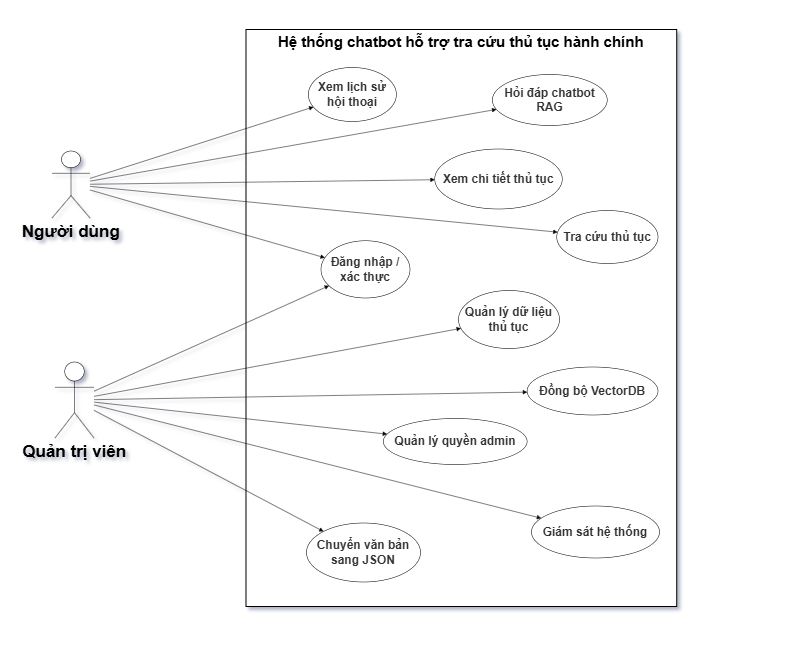
\includegraphics[width=0.92\textwidth]{tai_nguyen/media/image4.png}
\caption{Sơ đồ Use Case tổng quát của hệ thống}
\label{fig:2-4}
\end{figure}

Sơ đồ Use Case tổng quát thể hiện hai tác nhân chính và các chức năng
bắt buộc: tra cứu thủ tục, xem chi tiết thông tin thủ tục, hỏi đáp bằng
chatbot, lưu/xem lịch sử, quản lý dữ liệu thủ tục và quản lý hoạt động
hệ thống. Use Case ``Xem chi tiết thông tin thủ tục'' được tách riêng vì
đây là chức năng độc lập với luồng hỏi đáp chatbot.

\subsection{Sơ đồ Use Case nhóm người
dùng}
\begin{figure}[H]
\centering
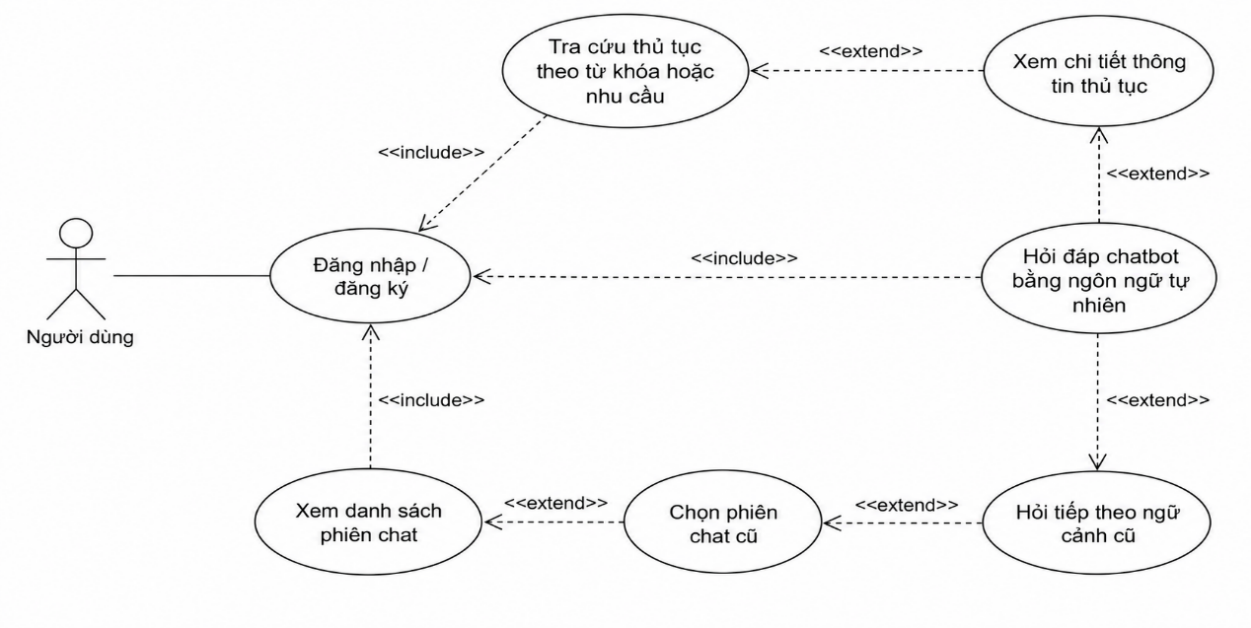
\includegraphics[width=0.92\textwidth]{tai_nguyen/media/image5.png}
\caption{Sơ đồ Use Case nhóm người dùng}
\label{fig:2-5}
\end{figure}

Nhóm Use Case của người dùng thể hiện rõ đường đi từ tra cứu đến xem chi
tiết và hỏi đáp. Người dùng có thể tìm thủ tục theo nhu cầu, mở thông
tin chi tiết, hỏi tiếp các trường cụ thể hoặc quay lại lịch sử hội thoại
đã lưu.

\subsection{Sơ đồ Use Case nhóm quản trị
viên}
\begin{figure}[H]
\centering
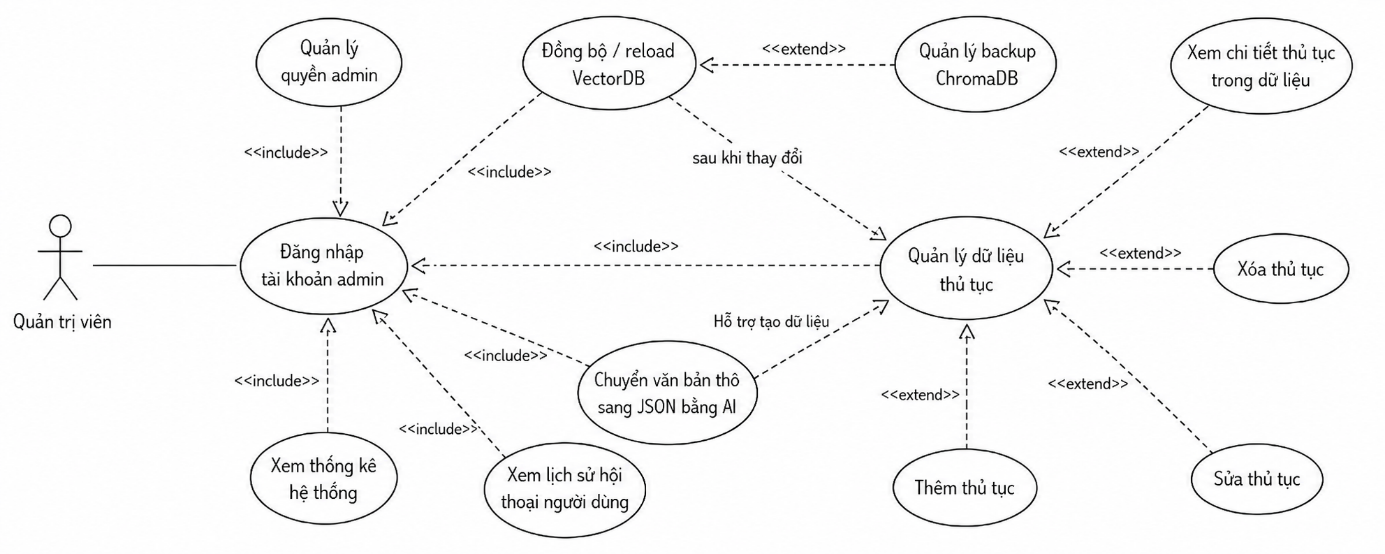
\includegraphics[width=0.92\textwidth]{tai_nguyen/media/image6.png}
\caption{Sơ đồ Use Case nhóm quản trị viên}
\label{fig:2-6}
\end{figure}

Nhóm Use Case của quản trị viên tập trung vào vận hành dữ liệu. Các chức
năng thêm/sửa/xóa thủ tục, chuyển văn bản sang JSON, đồng bộ VectorDB và
quản lý backup có tác động trực tiếp đến chất lượng kho tri thức, vì vậy
phải được bảo vệ bằng quyền admin ở backend.

\subsection{Đặc tả các Use Case
chính}

\begin{longtable}[]{|
  >{\raggedright\arraybackslash}p{(\columnwidth - 4\tabcolsep) * \real{0.1500}}|
  >{\raggedright\arraybackslash}p{(\columnwidth - 4\tabcolsep) * \real{0.4752}}|
  >{\raggedright\arraybackslash}p{(\columnwidth - 4\tabcolsep) * \real{0.3749}}|}
\caption{Tác nhân và Use Case chính}\\
\hline
\begin{minipage}[b]{\linewidth}\raggedright
\textbf{Tác nhân}
\end{minipage} & \begin{minipage}[b]{\linewidth}\raggedright
\textbf{Use Case chính}
\end{minipage} & \begin{minipage}[b]{\linewidth}\raggedright
\textbf{Vai trò}
\end{minipage} \\
\hline
\endfirsthead
\continuedcaption{Tác nhân và Use Case chính}
\hline
\begin{minipage}[b]{\linewidth}\raggedright
\textbf{Tác nhân}
\end{minipage} & \begin{minipage}[b]{\linewidth}\raggedright
\textbf{Use Case chính}
\end{minipage} & \begin{minipage}[b]{\linewidth}\raggedright
\textbf{Vai trò}
\end{minipage} \\
\hline
\endhead
\hline
\endlastfoot
Người dùng & UC01 Đăng nhập; UC02 Tra cứu thủ tục; UC03 Xem chi tiết thủ
tục; UC04 Hỏi đáp chatbot; UC05 Xem lịch sử & Tìm hiểu thông tin thủ tục
và quản lý lịch sử hỏi đáp cá nhân. \\
\hline
Quản trị viên & UC06 Quản lý dữ liệu; UC07 Đồng bộ VectorDB; UC08 Quản
lý admin; UC09 Chuyển văn bản sang JSON; UC10 Giám sát hệ thống & Vận
hành kho dữ liệu và theo dõi hoạt động chatbot. \\
\hline
Firebase Auth & Xác thực token & Cung cấp định danh để backend kiểm tra
quyền truy cập. \\
\hline
Firestore & Lưu sessions, messages, OTP, settings & Lưu dữ liệu nghiệp
vụ và cấu hình. \\
\hline
ChromaDB & Truy xuất vector & Lưu embedding và metadata của các chunk
thủ tục. \\
\hline
LLM & Sinh câu trả lời, hỗ trợ JSON & Diễn giải context RAG và hỗ trợ
admin tạo dữ liệu ban đầu. \\
\hline
\end{longtable}

\begin{longtable}[]{|
  >{\raggedright\arraybackslash}p{(\columnwidth - 2\tabcolsep) * \real{0.1559}}|
  >{\raggedright\arraybackslash}p{(\columnwidth - 2\tabcolsep) * \real{0.8441}}|}
\caption{Đặc tả UC01 - Đăng nhập và xác thực người dùng}\\
\hline
\begin{minipage}[b]{\linewidth}\raggedright
\textbf{Mục}
\end{minipage} & \begin{minipage}[b]{\linewidth}\raggedright
\textbf{Nội dung}
\end{minipage} \\
\hline
\endfirsthead
\continuedcaption{Đặc tả UC01 - Đăng nhập và xác thực người dùng}
\hline
\begin{minipage}[b]{\linewidth}\raggedright
\textbf{Mục}
\end{minipage} & \begin{minipage}[b]{\linewidth}\raggedright
\textbf{Nội dung}
\end{minipage} \\
\hline
\endhead
\hline
\endlastfoot
Tác nhân chính & Người dùng, Firebase Authentication, Backend
FastAPI. \\
\hline
Mục tiêu & Người dùng truy cập hệ thống bằng tài khoản hợp lệ và có
token để gọi API cần bảo vệ. \\
\hline
Tiền điều kiện & Người dùng có tài khoản Google/email; backend đã cấu
hình Firebase Admin SDK. \\
\hline
Luồng chính & \begin{minipage}[t]{\linewidth}\raggedright
1. Người dùng chọn phương thức đăng nhập.\\
2. Firebase xác thực tài khoản.\\
3. Frontend nhận ID Token.\\
4. Frontend gửi Bearer Token khi gọi API.\\
5. Backend xác minh token và cho phép truy cập.\strut
\end{minipage} \\
\hline
Ngoại lệ & 3.1Token hết hạn, sai định dạng hoặc tài khoản không tồn tại
thì backend từ chối request. \\
\hline
Hậu điều kiện & Người dùng vào giao diện chatbot và có thể lưu lịch sử
hội thoại. \\
\hline
\end{longtable}

\begin{longtable}[]{|
  >{\raggedright\arraybackslash}p{(\columnwidth - 2\tabcolsep) * \real{0.1403}}|
  >{\raggedright\arraybackslash}p{(\columnwidth - 2\tabcolsep) * \real{0.8597}}|}
\caption{Đặc tả UC02 - Tra cứu TTHC}\\
\hline
\begin{minipage}[b]{\linewidth}\raggedright
\textbf{Mục}
\end{minipage} & \begin{minipage}[b]{\linewidth}\raggedright
\textbf{Nội dung}
\end{minipage} \\
\hline
\endfirsthead
\continuedcaption{Đặc tả UC02 - Tra cứu TTHC}
\hline
\begin{minipage}[b]{\linewidth}\raggedright
\textbf{Mục}
\end{minipage} & \begin{minipage}[b]{\linewidth}\raggedright
\textbf{Nội dung}
\end{minipage} \\
\hline
\endhead
\hline
\endlastfoot
Tác nhân chính & Người dùng, Backend, dữ liệu
procedures.json/ChromaDB. \\
\hline
Mục tiêu & Người dùng tìm thủ tục liên quan khi chỉ biết từ khóa hoặc
nhu cầu thực tế. \\
\hline
Tiền điều kiện & Kho dữ liệu thủ tục đã được nạp; frontend kết nối được
backend. \\
\hline
Luồng chính & \begin{minipage}[t]{\linewidth}\raggedright
1. Người dùng nhập từ khóa hoặc nhu cầu.\\
2. Hệ thống chuẩn hóa truy vấn.\\
3. Backend tìm thủ tục liên quan theo tên, biến thể từ khóa hoặc ngữ
nghĩa.\\
4. Frontend hiển thị danh sách hoặc thủ tục phù hợp nhất.\strut
\end{minipage} \\
\hline
Ngoại lệ & 3.1 Không tìm thấy thủ tục phù hợp thì hệ thống gợi ý người
dùng nhập rõ hơn. \\
\hline
Hậu điều kiện & Người dùng có thể chọn thủ tục để xem chi tiết hoặc hỏi
chatbot. \\
\hline
\end{longtable}

\begin{longtable}[]{|
  >{\raggedright\arraybackslash}p{(\columnwidth - 2\tabcolsep) * \real{0.1714}}|
  >{\raggedright\arraybackslash}p{(\columnwidth - 2\tabcolsep) * \real{0.8286}}|}
\caption{Đặc tả UC03 - Xem chi tiết thông tin thủ tục}\\
\hline
\begin{minipage}[b]{\linewidth}\raggedright
\textbf{Mục}
\end{minipage} & \begin{minipage}[b]{\linewidth}\raggedright
\textbf{Nội dung}
\end{minipage} \\
\hline
\endfirsthead
\continuedcaption{Đặc tả UC03 - Xem chi tiết thông tin thủ tục}
\hline
\begin{minipage}[b]{\linewidth}\raggedright
\textbf{Mục}
\end{minipage} & \begin{minipage}[b]{\linewidth}\raggedright
\textbf{Nội dung}
\end{minipage} \\
\hline
\endhead
\hline
\endlastfoot
Tác nhân chính & Người dùng, Frontend, Backend, procedures.json. \\
\hline
Mục tiêu & Hiển thị thông tin chi tiết của một thủ tục độc lập với luồng
hỏi đáp chatbot. \\
\hline
Tiền điều kiện & Thủ tục tồn tại trong dữ liệu nguồn hoặc được tìm thấy
qua tra cứu. \\
\hline
Luồng chính & \begin{minipage}[t]{\linewidth}\raggedright
1. Người dùng chọn một thủ tục.\\
2. Frontend yêu cầu thông tin chi tiết.\\
3. Backend trả các trường hồ sơ, cơ quan, thời hạn, phí/lệ phí, kết quả,
căn cứ pháp lý.\\
4. Frontend hiển thị theo từng nhóm thông tin.\strut
\end{minipage} \\
\hline
Ngoại lệ & 3.1 Nếu thủ tục không tồn tại, hệ thống thông báo không tìm
thấy dữ liệu. \\
\hline
Hậu điều kiện & Người dùng xem được thông tin đầy đủ và có thể tiếp tục
đặt câu hỏi về thủ tục đó. \\
\hline
\end{longtable}

\begin{longtable}[]{|
  >{\raggedright\arraybackslash}p{(\columnwidth - 2\tabcolsep) * \real{0.1715}}|
  >{\raggedright\arraybackslash}p{(\columnwidth - 2\tabcolsep) * \real{0.8285}}|}
\caption{Đặc tả UC04 - Hỏi đáp TTHC bằng chatbot}\\
\hline
\begin{minipage}[b]{\linewidth}\raggedright
\textbf{Mục}
\end{minipage} & \begin{minipage}[b]{\linewidth}\raggedright
\textbf{Nội dung}
\end{minipage} \\
\hline
\endfirsthead
\continuedcaption{Đặc tả UC04 - Hỏi đáp TTHC bằng chatbot}
\hline
\begin{minipage}[b]{\linewidth}\raggedright
\textbf{Mục}
\end{minipage} & \begin{minipage}[b]{\linewidth}\raggedright
\textbf{Nội dung}
\end{minipage} \\
\hline
\endhead
\hline
\endlastfoot
Tác nhân chính & Người dùng, Backend, ChromaDB, Reranker, LLM. \\
\hline
Mục tiêu & Người dùng đặt câu hỏi tự nhiên và nhận câu trả lời dựa trên
dữ liệu đã truy xuất. \\
\hline
Tiền điều kiện & Backend đã khởi động; vector database đã được load hoặc
build thành công. \\
\hline
Luồng chính & \begin{minipage}[t]{\linewidth}\raggedright
1. Người dùng nhập câu hỏi.\\
2. Frontend gửi request đến /user/chat.\\
3. Backend lấy lịch sử session.\\
4. Pipeline RAG truy xuất và rerank dữ liệu.\\
5. LLM sinh câu trả lời từ context.\\
6. Hệ thống trả kết quả và lưu lịch sử.\strut
\end{minipage} \\
\hline
Ngoại lệ & \begin{minipage}[t]{\linewidth}\raggedright
4.1 DB chưa sẵn sàng thì báo đang khởi tạo;\\
6.1 Không có dữ liệu phù hợp thì trả ``Dữ liệu hiện tại không đề
cập''.\strut
\end{minipage} \\
\hline
Hậu điều kiện & Câu hỏi và câu trả lời được lưu vào Firestore theo
session. \\
\hline
\end{longtable}

\begin{longtable}[]{|
  >{\raggedright\arraybackslash}p{(\columnwidth - 2\tabcolsep) * \real{0.1714}}|
  >{\raggedright\arraybackslash}p{(\columnwidth - 2\tabcolsep) * \real{0.8286}}|}
\caption{Đặc tả UC05 - Xem lịch sử hội thoại}\\
\hline
\begin{minipage}[b]{\linewidth}\raggedright
\textbf{Mục}
\end{minipage} & \begin{minipage}[b]{\linewidth}\raggedright
\textbf{Nội dung}
\end{minipage} \\
\hline
\endfirsthead
\continuedcaption{Đặc tả UC05 - Xem lịch sử hội thoại}
\hline
\begin{minipage}[b]{\linewidth}\raggedright
\textbf{Mục}
\end{minipage} & \begin{minipage}[b]{\linewidth}\raggedright
\textbf{Nội dung}
\end{minipage} \\
\hline
\endhead
\hline
\endlastfoot
Tác nhân chính & Người dùng, Frontend, Backend, Firestore. \\
\hline
Mục tiêu & Người dùng mở lại phiên chat đã lưu và tiếp tục hội thoại. \\
\hline
Tiền điều kiện & Người dùng đã đăng nhập và có session đã được tạo. \\
\hline
Luồng chính & \begin{minipage}[t]{\linewidth}\raggedright
1. Frontend gọi /user/sessions.\\
2. Backend truy vấn sessions theo uid.\\
3. Người dùng chọn session.\\
4. Frontend gọi /user/chat/history.\\
5. Tin nhắn được hiển thị theo thứ tự thời gian.\strut
\end{minipage} \\
\hline
Ngoại lệ & \begin{minipage}[t]{\linewidth}\raggedright
2.1 Không có session thì sidebar trống;\\
4.1 Lỗi Firestore thì hệ thống trả danh sách rỗng.\strut
\end{minipage} \\
\hline
Hậu điều kiện & Người dùng có thể tiếp tục hỏi trong session hiện
tại. \\
\hline
\end{longtable}

\begin{longtable}[]{|
  >{\raggedright\arraybackslash}p{(\columnwidth - 2\tabcolsep) * \real{0.1714}}|
  >{\raggedright\arraybackslash}p{(\columnwidth - 2\tabcolsep) * \real{0.8286}}|}
\caption{Đặc tả UC06 - Quản lý dữ liệu TTHC}\\
\hline
\begin{minipage}[b]{\linewidth}\raggedright
\textbf{Mục}
\end{minipage} & \begin{minipage}[b]{\linewidth}\raggedright
\textbf{Nội dung}
\end{minipage} \\
\hline
\endfirsthead
\continuedcaption{Đặc tả UC06 - Quản lý dữ liệu TTHC}
\hline
\begin{minipage}[b]{\linewidth}\raggedright
\textbf{Mục}
\end{minipage} & \begin{minipage}[b]{\linewidth}\raggedright
\textbf{Nội dung}
\end{minipage} \\
\hline
\endhead
\hline
\endlastfoot
Tác nhân chính & Quản trị viên, Backend FastAPI, procedures.json,
Firestore \\
\hline
Mục tiêu & Quản trị viên quản lý danh sách thủ tục hành chính trong hệ
thống, bao gồm thêm, sửa, xóa và kiểm tra dữ liệu trước khi đồng bộ kho
tri thức. \\
\hline
Tiền điều kiện & Tài khoản đã được cấp quyền admin; backend kết nối được
dữ liệu nguồn. \\
\hline
Luồng chính & 1. Quản trị viên truy cập giao diện quản lý dữ liệu.

2. Frontend gửi request lấy danh sách thủ tục.

3. Backend đọc dữ liệu từ procedures.json hoặc collection liên quan.

4. Quản trị viên thực hiện thêm, sửa hoặc xóa thủ tục.

5. Backend kiểm tra dữ liệu đầu vào.

6. Hệ thống lưu dữ liệu mới và cập nhật metadata cần thiết. \\
\hline
Ngoại lệ & \begin{minipage}[t]{\linewidth}\raggedright
5.a Dữ liệu thiếu trường bắt buộc hoặc sai cấu trúc thì hệ thống từ chối
lưu.\\
6.a File dữ liệu đang bị khóa hoặc lỗi ghi thì backend trả thông báo
thất bại.\strut
\end{minipage} \\
\hline
Hậu điều kiện & Dữ liệu thủ tục được cập nhật và sẵn sàng cho quá trình
build lại VectorDB. \\
\hline
\end{longtable}

\begin{longtable}[]{|
  >{\raggedright\arraybackslash}p{(\columnwidth - 2\tabcolsep) * \real{0.1714}}|
  >{\raggedright\arraybackslash}p{(\columnwidth - 2\tabcolsep) * \real{0.8286}}|}
\caption{Đặc tả UC07 - Đồng bộ và xây dựng lại VectorDB}\\
\hline
\begin{minipage}[b]{\linewidth}\raggedright
\textbf{Mục}
\end{minipage} & \begin{minipage}[b]{\linewidth}\raggedright
\textbf{Nội dung}
\end{minipage} \\
\hline
\endfirsthead
\continuedcaption{Đặc tả UC07 - Đồng bộ và xây dựng lại VectorDB}
\hline
\begin{minipage}[b]{\linewidth}\raggedright
\textbf{Mục}
\end{minipage} & \begin{minipage}[b]{\linewidth}\raggedright
\textbf{Nội dung}
\end{minipage} \\
\hline
\endhead
\hline
\endlastfoot
Tác nhân chính & Quản trị viên, Backend FastAPI, ChromaDB, Embedding
Model \\
\hline
Mục tiêu & Đồng bộ lại kho vector sau khi dữ liệu thủ tục thay đổi nhằm
đảm bảo chatbot truy xuất đúng dữ liệu mới nhất. \\
\hline
Tiền điều kiện & Dữ liệu procedures.json hợp lệ; embedding model và
ChromaDB đã được khởi tạo. \\
\hline
Luồng chính & 1. Quản trị viên chọn chức năng đồng bộ VectorDB.

2. Backend kiểm tra dữ liệu JSON đầu vào.

3. Hệ thống backup thư mục ChromaDB hiện tại.

4. Backend thực hiện chunking dữ liệu thủ tục.

5. Embedding model sinh vector cho từng chunk.

6. Hệ thống nạp vector và metadata vào ChromaDB mới.

7. Backend lưu database mới xuống bộ nhớ.

8. Hệ thống trả trạng thái build thành công. \\
\hline
Ngoại lệ & 2.a JSON không hợp lệ thì dừng quá trình đồng bộ.

5.a Embedding model lỗi hoặc hết tài nguyên RAM thì quá trình build bị
hủy.

6.a Không ghi được dữ liệu xuống ChromaDB thì rollback về bản backup
trước đó. \\
\hline
Hậu điều kiện & Kho vector mới được kích hoạt và chatbot sử dụng dữ liệu
đã cập nhật cho các truy vấn tiếp theo. \\
\hline
\end{longtable}

Các Use Case quản trị gồm quản lý dữ liệu thủ tục, đồng bộ VectorDB,
quản lý quyền admin, chuyển văn bản sang JSON và giám sát hệ thống. Các
Use Case này được bảo vệ bằng quyền admin ở backend vì có thể tác động
trực tiếp đến dữ liệu nguồn, lịch sử hội thoại hoặc kho vector của hệ
thống.

\section{Tổng hợp phân tích và lựa chọn giải
pháp
RAG}

Từ các phần khảo sát, phân tích dữ liệu, phạm vi hệ thống, tác nhân, quy
trình nghiệp vụ và yêu cầu hệ thống, có thể thấy bài toán tra cứu TTHC
cần một giải pháp vừa hiểu được ngôn ngữ tự nhiên vừa bám dữ liệu nguồn.
Nếu chỉ dùng tìm kiếm từ khóa, hệ thống khó xử lý các câu hỏi đời thường
hoặc câu hỏi không nêu đúng tên thủ tục. Nếu chỉ dùng LLM thuần túy, câu
trả lời có thể trôi khỏi dữ liệu hành chính công và khó kiểm chứng.

So với chatbot rule-based, RAG linh hoạt hơn khi người dân diễn đạt khác
mẫu câu. So với LLM thuần túy, RAG an toàn hơn vì câu trả lời bị ràng
buộc bởi dữ liệu nguồn. Vì vậy, RAG là phương án phù hợp nhất với mục
tiêu của đề tài: hỗ trợ tra cứu bằng ngôn ngữ tự nhiên nhưng vẫn giữ
được căn cứ dữ liệu hành chính công.

\begin{longtable}[]{|
  >{\raggedright\arraybackslash}p{(\columnwidth - 6\tabcolsep) * \real{0.1582}}|
  >{\raggedright\arraybackslash}p{(\columnwidth - 6\tabcolsep) * \real{0.2424}}|
  >{\raggedright\arraybackslash}p{(\columnwidth - 6\tabcolsep) * \real{0.2401}}|
  >{\raggedright\arraybackslash}p{(\columnwidth - 6\tabcolsep) * \real{0.3592}}|}
\caption{So sánh các giải pháp chatbot cho bài toán tra cứu TTHC}\\
\hline
\begin{minipage}[b]{\linewidth}\raggedright
\textbf{Tiêu chí}
\end{minipage} & \begin{minipage}[b]{\linewidth}\raggedright
\textbf{Rule-based chatbot}
\end{minipage} & \begin{minipage}[b]{\linewidth}\raggedright
\textbf{LLM thuần túy}
\end{minipage} & \begin{minipage}[b]{\linewidth}\raggedright
\textbf{Chatbot RAG đề xuất}
\end{minipage} \\
\hline
\endfirsthead
\continuedcaption{So sánh các giải pháp chatbot cho bài toán tra cứu TTHC}
\hline
\begin{minipage}[b]{\linewidth}\raggedright
\textbf{Tiêu chí}
\end{minipage} & \begin{minipage}[b]{\linewidth}\raggedright
\textbf{Rule-based chatbot}
\end{minipage} & \begin{minipage}[b]{\linewidth}\raggedright
\textbf{LLM thuần túy}
\end{minipage} & \begin{minipage}[b]{\linewidth}\raggedright
\textbf{Chatbot RAG đề xuất}
\end{minipage} \\
\hline
\endhead
\hline
\endlastfoot
Cơ chế & So khớp từ khóa và kịch bản cố định. & Sinh câu trả lời từ kiến
thức mô hình. & Truy xuất dữ liệu liên quan rồi sinh câu trả lời từ
context. \\
\hline
Hiểu ngôn ngữ tự nhiên & Hạn chế, phụ thuộc mẫu câu. & Tốt nhưng khó
kiểm soát nguồn. & Tốt, kết hợp semantic search và LLM. \\
\hline
Độ chính xác hành chính & Đúng khi khớp kịch bản, khó mở rộng. & Không
ổn định, có nguy cơ hallucination. & Cao hơn vì bị ràng buộc bởi dữ liệu
nguồn. \\
\hline
Cập nhật dữ liệu & Phải sửa luật/kịch bản. & Có thể cần fine-tune hoặc
phụ thuộc dữ liệu huấn luyện. & Cập nhật JSON và build lại vector
database. \\
\hline
Khả năng mở rộng & Kém khi số thủ tục tăng. & Phụ thuộc chi phí mô hình.
& Phù hợp hơn với kho dữ liệu lớn có metadata. \\
\hline
\end{longtable}

Lựa chọn RAG cũng phù hợp với khả năng cập nhật dữ liệu của hệ thống.
Khi thủ tục thay đổi, quản trị viên có thể cập nhật dữ liệu JSON và
build lại VectorDB thay vì phải viết lại toàn bộ kịch bản hỏi đáp. Đây
là điểm quan trọng đối với hệ thống hành chính công, nơi dữ liệu có thể
thay đổi theo văn bản pháp lý mới.
